% LaTeX file for Chapter 02


\chapter{Methodology} 

\section{Definitions}

The \textit{Target Population} is a specific group within the broader population, defined by attributes relevant to the research question. This group is selected based on criteria that match the study's goals, helping researchers focus on the most pertinent segments of the population \citep{willie2024population}. Defining the target population allows researchers to refine their objectives and sampling methods to align with the study's aims.


The \textit{Eligibility} criteria are the specific requirements that individuals must meet to participate in a study. Eligible patients will be selected from the target population. It is important to note that eligibility criteria also include exclusion factors, conditions or circumstances that disqualify potential participants \citep{food2018evaluating}. Inclusion criteria specify the conditions that allow individuals to participate in the trial, particularly focusing on the medical condition of interest. Any other factors that limit eligibility are classified as exclusion criteria \citep{van2007eligibility}.


In clinical trials, \textit{Enrollment} refers to the formal process of registering participants into a study after they have met all eligibility criteria and provided informed consent. This process includes verifying that each participant satisfies the inclusion and exclusion criteria outlined in the study protocol \citep{NIH2021}. It is important to distinguish between recruitment and enrollment. Recruitment involves identifying and inviting potential participants to join the study, whereas enrollment occurs after these individuals have been screened, consented, and officially registered into the trial \citep{frank2004current}. 

Once enrolled, participants are assigned to specific treatment groups or interventions as defined by the study design. The most common practice been \textit{Randomization}. In clinical research, randomization is the process of assigning participants to different treatment groups using chance methods, such as random number generators or coin flips \citep{lim2019randomization}. Randomized controlled trials (RCTs) are considered the most effective method for preventing bias in the evaluation of new interventions, drugs, or devices. \citep{van2007eligibility}.


% $T=time$
% $C=counts$
% $\lambda=\frac{C}{T}$
% \begin{tabular}{|c|c|c|c|c|}
%     \hline
%      & \textbf{Expectation} & \textbf{SD} & \textbf{Aleatory Uncertainty} & \textbf{Epistemic Uncertainty} \\ \hline
%     Point Estimate & $\lambda\cdot T$ & 0 & NO & NO \\ \hline
%     $C\sim Poi(\lambda)$ & $\lambda\cdot T$ & $\lambda\cdotT$ & YES & NO \\ \hline
%     $C\sim Poi(\Lambda)$ with $\Lambda\sim Gamma (\alpha,\beta)$& [...] & [...] & YES & YES \\ \hline
% 
% \end{tabular}



\hrule





\hrule

\bigskip 

This options are best placed in the main document at the beginning. Otherwise a \verb+cache=FALSE+ as knitr option is necessary to overrule a possible  \verb+cache=TRUE+ flag. 

\bigskip 

Notice how in Figure~\ref{f02:1} everything is properly scaled.   

\begin{figure}
\begin{knitrout}
\definecolor{shadecolor}{rgb}{0.98, 0.98, 0.98}\color{fgcolor}

{\centering 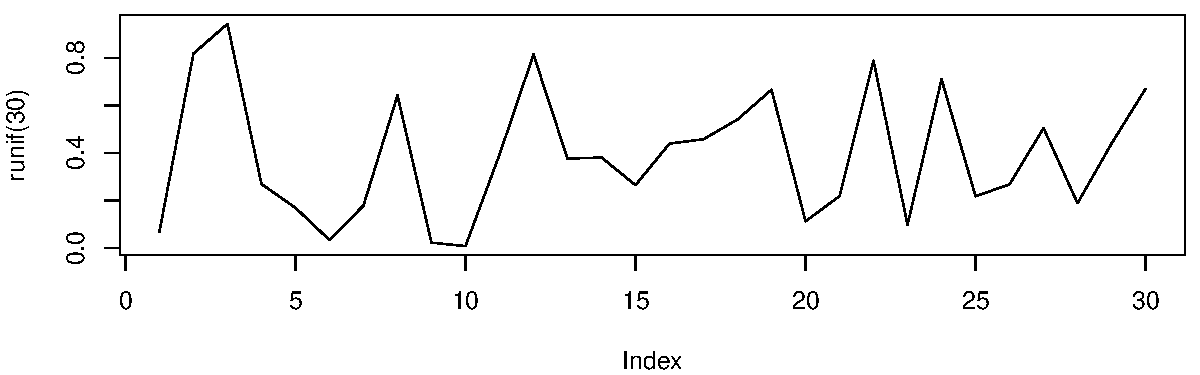
\includegraphics[width=\textwidth-3cm]{figure/ch02_figunnamed-chunk-3-1} 

}


\end{knitrout}
  \caption{Test figure to illustrate figure options used by knitr.}
  \label{f02:1}
\end{figure}


\section{Citations}

Recall the difference between \verb+\citet{}+ (e.g., \citet{Chu:Geor:99}), \verb+\citep{}+ (e.g., \citep{Chu:Geor:99}) and \verb+\citealp{}+ (e.g., \citealp{Chu:Geor:99}).
For simplicity, we include here all references in the file \verb+biblio.bib+ with the command \verb+\nocite{*}+.\nocite{*}

